% Todo: Introduction structure
% 0) we introduce & define the problem 1) we survey which techniques
exist 2) we implement (for a lack of readily available implementations)
and compare the most promising ones 3) we draw conclusions for when to
use which technique


% TODO: Include term predictive CI, link to FB paper and
https://www-sciencedirect-com.tudelft.idm.oclc.org/science/article/pii/S0164121218301730

% TODO: What about the alternate solution, installing plugins to report
precise data? Ie., maven plugins
% - Lots of effort
% - not a generic solution
% - how to analyze history where such plugins were not installed
% - unclear which information you want

% TODO It would be futile to compare our techniques with one of the
existing manual regex parsers, as (a) as our literature survey showed,
their scope is mainly limited to the Java ecosystem and (b) whether
they would work or not would be randomly based on whether the project
we select exhibits features their regular expressions were trained for.
Finally, they are not really automatic

\lstset{
  morekeywords={},
	basicstyle=\ttfamily\scriptsize,
  postbreak=\mbox{\textcolor{blue}{$\hookrightarrow$}\space},
  showspaces=false,
  showstringspaces=false,
  stringstyle=\color{Plum},
	frame=single,
  extendedchars=false,
  texcl=false,
  aboveskip=\baselineskip,
  belowskip=0pt
}

Continuous Integration (CI) has become a common practice in software
engineering~\cite{hilton2016usage}.
Many software projects use
CI~\cite{hilton2016usage,staahl2014modeling,beller2017oops} to detect
bugs early~\cite{vasilescu2015quality,duvall2007continuous}, improve
developer productivity~\cite{miller2008hundred,hilton2016usage} and
communication~\cite{downs2012ambient}.
CI builds produce logs which
report results of various sub-steps within the build.
These build logs
contain a lot of valuable information for developers and researchers---for
example, descriptions of compile errors, linter warnings or failed
tests~\cite{beller2017oops,seo2014programmers,vassallo2017a-tale}.

CI builds produce logs which report the results of the steps within
the build.
The information stored in build logs can and has
already been used for a variety of applications.
One prominent dataset
in the space, TravisTorrent, was featured as the MSR Data Challenge
2017~\cite{msr17challenge}.
To date, scientist and practitioners alike
have used it and other, proprietary datasets to understand and
cateogrize Continuous Integration build
failures~\cite{islam2017insights}, to do research on testing
practices~\cite{orellana2017differences}, to train classifiers to
predict the build outcome and
duration~\cite{ni2017cost,bisong2017built,machalica2019predictive},
and to investigate static analysis tools in CI
builds~\cite{zampetti2017open}.
Therefore, being able to efficiently
and correctly extract information from build logs is paramount to the
future of a variety of fields depending on it.

However, build logs can be verbose and large---sometimes in excess of
50 MB of ASCII text ~\cite{beller2017oops}---making them inadequate
for direct human consumption.
Therefore, to support developers and
researchers in efficiently making use of the information within build
logs, we must at least semi-automatically retrieve the chunks of the
log that describe the targeted information.

There are different techniques to retrieve information chunks from CI
build logs.
Beller et al.
use a rule-based system of regular
expressions to analyze logs from Travis CI~\cite{beller2017oops}.
Such regular expressions are developed by looking at exemplary build
logs.
Vassallo et al.\ wrote a custom parser to gather information
for build repair hints~\cite{vassallo2018un-break}.
Recently, Amar et
al.\ reduced the number of lines for a developer to inspect by
creating a diff between logs from failed and successful
builds~\cite{amar2019mining}.

These approaches have various strengths and weaknesses: Regular
expressions are exact, but tedious and error-prone to
maintain~\cite{michael2019regexes}.
Custom parsers are powerful
though fragile in light of changes in the log structure.
Diffing
between failed and successful logs can reduce the information to be
processed, but is at best semi-automatic~\cite{amar2019mining}.

To gain an impression on how researchers are using information from
build logs
within their research and how they are gathering chunks from them
to support
developers in understanding build outcomes, we conducted a systematic
mapping
study.
Our goal was to classify how and what for researchers use build logs as
a source
of data (\textbf{RQ1}).

The outcomes of our study shows that there are various attempts to
retrieve
specific information from buildlogs.
The resulting implementations are rarely
available and therefore rarely reused.
Because of the high development overhead
of the custom parsers, many implementations are limited to small number
of supported
build tools.

To address this, we implement three promising techniques for build
log analysis.
They retrieve specific chunks of targeted information and are configured
by
examples provided by the user.
We conduct an empirical study on the \emph{LogChunks} data
set~\cite{brandt2020logchunks} to
gauge the performance of these chunk retrieval techniques and characterize
when one of the techniques should be preferred over other alternatives
(\textbf{RQ2}).

\begin{simplebox}{Research Questions}
\begin{itemize}
  \item[\textbf{RQ1:}] Which build log analysis techniques exist?
  \item[\textbf{RQ2:}] Which criteria influence the suitability of a chunk
  retrieval technique for build logs?
\end{itemize}
\end{simplebox}

% At the moment there is only anecdotal evidence on the performance
of these
% techniques and on when a technique should be preferred over other
alternatives.
% Developers and researches currently have little support when choosing
which
% technique to use for a task.

% The goal of this article is to investigate different chunk retrieval
techniques
% for build logs and describe under which circumstances certain techniques
can be
% recommended over others.
% We aim to characterize different chunk retrieval techniques.
% For \textbf{Research Question 1} (\textbf{RQ1}), we analyze which
criteria
% influence the suitability of a chunk retrieval technique for CI
build logs.

We implement and evaluate three chunk retrieval techniques:
\begin{itemize}
  \item \textbf{Program Synthesis by Example (referred to as PBE)}
  Based on user examples of build logs and targeted log chunks, PBE
  synthesizes
  a regular expression matching the given chunks within the build logs.
  \item \textbf{Common Text Similarity (CTS)}
  Using the Vector Space Model, CTS selects those lines of a log which are
  most similar to the lines present in example chunks provided by
  the user.
  \item \textbf{Keyword Search (KWS)}
  Ad-hoc method for finding fitting passages by searching the whole
  text for
  the occurrence of specific trigger words.
\end{itemize}

\begin{figure}[!t]
  \centering
  \begin{lstlisting}[breaklines=true,frame=tlr]
FAILURE: Build failed with an exception.

* What went wrong:
  \end{lstlisting}
  \vspace{-\baselineskip}
  \begin{lstlisting}[backgroundcolor=\color{Cerulean!60},breaklines=true,frame=rl]
Could not determine the dependencies of task `:app:jacocoTestDebugReport'.
> Task with path 'testDebug' not found in project ':app'.
  \end{lstlisting}
  \vspace{-\baselineskip}
  \begin{lstlisting}[breaklines=true,frame=blr]

* Try:
  \end{lstlisting}
  \caption{Example of a log chunk explaining why an Android/Gradle
  build failed.}
  % TODO Moritz: we can relate this to travistorrent maybe, you told me
  long ago that this was something your analyzer cannot extract
  \label{lst:chunk-example-1}
\end{figure}

\begin{figure}[!t]
  \centering
  \begin{lstlisting}[breaklines=true,frame=tlr]
FAILURE: Build failed with an exception.

* What went wrong:
  \end{lstlisting}
  \vspace{-\baselineskip}
  \begin{lstlisting}[backgroundcolor=\color{Cerulean!60},breaklines=true,frame=rl]
Execution failed for task ':app:connectedAndroidTest'.
> com.android.builder.testing.api.DeviceException:
java.lang.RuntimeException: ...
  \end{lstlisting}
  \vspace{-\baselineskip}
  \begin{lstlisting}[breaklines=true,frame=blr]

* Try:
  \end{lstlisting}
  \caption{Another example of a log chunk explaining why an Android/Gradle
  build failed.}
  \label{lst:chunk-example-2}
\end{figure}

\lstset{language=caml, morekeywords={StartExtraction, RegexPosition,
RegexPair,
  EndExtraction}, keywordstyle=\bfseries\color{black}, escapeinside=//}
\begin{figure}[!t]
  \centering
  \begin{lstlisting}[breaklines=true]
StartExtraction(RegexPair("Colon/{\color{Plum}$\circ$}/Line Separator",
"ALL CAPS")) in EndExtraction(RegexPair("/{\color{Plum}$\varepsilon$}/",
"Line Separator/{\color{Plum}$\circ$}/Line Separator"))
  \end{lstlisting}
  \caption{Simiplified regular expression produced by PBE when trained
  with examples from \Cref{lst:chunk-example-1,lst:chunk-example-2}}
  \label{lst:prose-program-simplified}
\end{figure}

\lstset{
  language=,
  morekeywords={},
  texcl=false
}
\begin{figure}[!t]
  \centering
  \begin{lstlisting}[breaklines=true,frame=tlr]
=== RUN   TestSeparator
  \end{lstlisting}
  \vspace{-\baselineskip}
  \begin{lstlisting}[backgroundcolor=\color{Cerulean!60},breaklines=true,frame=rl]
--- FAIL: TestSeparator (0.03s)
    repo\_test.go:75: expected entry to be in form of `* [link] -
    description.`, got '* ...
  \end{lstlisting}
  \vspace{-\baselineskip}
  \begin{lstlisting}[breaklines=true,frame=blr]
=== RUN   TestGenerateHTML
  \end{lstlisting}
  \caption{Example of a log chunk.
%\todo{which build tool?}
%  \todo{move to where structural category explanation}
}
  \label{lst:chunk-example-3}
\end{figure}

The results of our empirical comparison study on the chunk retrieval
techniques
show that the structural representation of the targeted chunk greatly
influences
the performance of the chunk retrieval techinques.
\Cref{lst:chunk-example-1,lst:chunk-example-2} show two exemplary
log chunks
from Android/Gradle build logs marked in blue.
Both chunks contain the information on why the
corresponding build failed.
When PBE is trained on these two examples it produces
a regular expression similar to \Cref{lst:prose-program-simplified}.
The retrieval
starts after a colon followed by a line separator and before a capital
letter.
It ends before two line separators, consistent with the two example
chunks from
\Cref{lst:chunk-example-1,lst:chunk-example-2}.
This shows, that the characters structuring the text around the chunk are
cruicial for regular expressions to identify the targeted log chunk.
In fact, if the third
example from \Cref{lst:chunk-example-3} with a different structural
representation is added, PBE is not able to syntesize a program and
returns
``\texttt{no program found}''.
We express this difference in structural representation through
dividing log
chunks into structural categories.
The chunks from
\Cref{lst:chunk-example-1,lst:chunk-example-2} are in the same structural
category, while the chunk from \Cref{lst:chunk-example-3} is in a
different one.


% \textbf{RQ2} asks under which conditions PBE, CTS and KWS are suited
to retrieve information from continuous integration build logs.
% \textbf{RQ2} is refined into sub-questions along with the criteria
resulting from \textbf{RQ1} and compares their instantiations for the
three techniques:
% how many training examples a technique needs to perform best
(\textbf{RQ2.1}), how structurally diverse the examples can
be (\textbf{RQ2.2}) and how accurate the retrieved output is
(\textbf{RQ2.3}).
% To evaluate PBE, CTS and KWS we use the \emph{LogChunks} data set,
which encompasses about 800 log files from 80 repositories.
% Each log is labeled with the log part describing the reason a build
failed, keywords to search for this log part and a categorization of
the labeled log part according to its structural representation within
the log.

Our study of the three techniques on \emph{LogChunks} shows that
\begin{itemize}
  \item PBE yields very accurate results when trained with two examples
  from a
  single structural category.
  \item CTS shows the best average precision, though precision and recall
  of a
  retrieval is hard to determine from the given result.
  A small increase in the number of training examples has no noticeable
  influence.

  Fewer structural categories improve precision and recall of the
  retrieval.
  \item KWS has the highest recall of all techniques, however much
  lower precision.
  It is the technique with the best recall when multiple structural
  categories
  are present in the training examples.
\end{itemize}

% \noindent
% \textbf{Our work contributes:}
% \begin{itemize}
%   \item A tool with three prototypical implementations of chunk
retrieval techniques:
%	  \begin{itemize}
%	    \item program synthesis from examples using the Microsoft
PROSE library (PBE),
%	    \item a common information retrieval approach using text
similarity (CTS), and
%	    \item a keyword search approach (KWS).
%	  \end{itemize}
%   \item Recommendations for the configuration of each of the
investigated chunk retrieval techniques.
%   \item Guidelines on choosing a suitable chunk retrieval technique.
% \end{itemize}

We recommend PBE for use cases where the desired information is always
represented in the same structural way and high confidence in precision
and
recall of the chunk retrieval is required.
CTS is well suited when the representation of the desired information
varies
slightly and the output of the chunk retrieval is further processed by
a human.
In cases where the textual representation of the desired information in
the log
is unpredictable or varies greatly, KWS seems to be the best choice.
However,
its low precision---it extracts a context of multiple lines around a
finding---makes it generally unsuited for automatic on-ward processing and
instead requires a human to further inspect and interpret the output
chunk.

\section{Related Work}
% TODO reorder rw by build retrieval technique rather than by paper
\label{sec:rw}
We explain how researchers gather information about CI usage in software
projects
through build log analysis and why the chunk retrieval techniques we
investigate
simplifies their data collection.
This section moves on to past works about augmenting build logs to make
it easier
for developers to inspect them.
The presented approaches are related to and can benefit from the
techniques we
analyze in this article.
Further, we classify build logs as semi-structured data and differentiate
our
work from system log analysis.

\subsection{Build Failures in CI}
Various researchers studied why CI builds fail and into the impact of
build failures on the development workflow.

Seo et al.~\cite{seo2014programmers} find that a small group of error
types such as dependency mismatches are the most prominent cause of
build failures at Google.
In addition, they notice that most failures
are resolved within two builds.
They based their analyses on sets of
build logs collected from industry partners.
They develop a custom
parser to classify error messages reported by Java and C++ builds.

Rausch et al.~\cite{rausch2017empirical} analyze CI builds of open
source Java projects and find that most builds fail because of failing
tests.
For most projects, over half of the failed builds follow a
previous failed build.
Rausch et al.'s data shows that most failures
occur in the second half of the build runtime, which can cause long
delays in the feedback loop, especially when builds are automatically
retried upon failure.

Vassallo et al.~\cite{vassallo2017a-tale} compare open source projects
in Java to industrial ones.
They determine that testing failures are
more common than compilation errors.
Open source builds fail most
often because of unit tests, whereas release preparations are the
primary cause in industrial projects.
Their data stems from analyzing
build logs from \emph{TravisTorrent}~\cite{beller2017travistorrent}
with regular expressions.

Ghaleb et al.~\cite{ghaleb2019studying} aim to identify noise in build
breakage data.
They classify build failures from \emph{TravisTorrent}
according to whether they were caused by an environmental failure or
caused by a developer change.
Their analysis starts with manual
categorization of build logs.
They select keywords and strings that
identify their targeted categories and code a script to automatically
classify logs based on these keywords.

\noindent
\textbf{Supporting Log Analysis with Chunk Retrieval}
To leverage the valuable information within build logs the researchers
presented in this section create parsers and regular expression-based
programs.
This task of retrieving specific chunks of text from the
build logs can be solved by the chunk retrieval techniques we compare
in this article.
Our results can support researchers in choosing a
suitable technique for their data set of build logs and the chunks
they want to retrieve.
By relieving them from building custom parsers
we enable them to cover a much wider range of languages and build
tools in their studies.


\subsection{Augmentation of Build Logs}
\label{sec:rw-bl-analysis}
Build logs are a valuable data source for developers to find out why
their build failed.
Several researchers investigate how to support
developers in working with verbose build logs.
Vassallo et
al.~\cite{vassallo2018un-break} try to shorten the time it takes
developers to understand build logs.
They parse
Maven~\cite{maven2019website} build logs into a structured
representation and create hint generators.
%The hint generators leverage this structured access to the
%information within the build log to propose fixes.
For example, one of the hint generators queries stack overflow for
discussions related to why the build failed.
In a qualitative study
they observed that highlighting the locality and context of an issue
is helpful to programmers.
%Their tool BART is published as a Jenkins
%Plugin~\cite{bart2019plugin}.
The chunk retrieval techniques we compare in this article can be used
to fill similar structured representations with information from build
logs.
As they simplify the construction of parsers they would enable
developers and researchers to cover a wider array of build tools,
which is the main influence factor on the structure of a build log.

Amar et al.~\cite{amar2019mining} compare different approaches to
reduce the portions of a log that a developer has to inspect.
Their
techniques remove lines that appear both in logs from passing and
failing builds and use a modified \emph{Term Frequency Inverse
Document Frequency} (TF-IDF) weighting to identify term vectors likely
to occur with failures.
Their diff technique can be interpreted as a
chunk retrieval technique, where the targeted information is defined
by the past failures used as basis for the weighted term vectors.

Travis itself already provides build log augmentation in the form of a
basic structuring of the build logs within their log viewer using
\emph{log folds}~\cite{travis2019logfolds}.
They add fold identifiers
around common commands and setup or teardown build phases and collapse
the contained lines by default.

\subsection{System Log Analysis}
\label{sec:log-analysis}
A related field of log processing is the processing of system log
files produced during runtime.
A main difference between build logs
and system logs is that system logs are fundamentally structured
through events.
Each line in a log file represents one event with a
set of fields: timestamp, verbosity level and raw message
content~\cite{he2017towards}.
Figure \ref{lst:system-log} shows
example lines from a system log.

The first goal in analyzing system log files is ubiquitously to
separate constant and variable parts within a log
message~\cite{nagappan2010abstracting,he2017towards}.
Next, the log
messages are clustered into log events, unifying messages with
identical constant parts and varying parameters.
The output of a log
parser is an ordered list of timed events and their corresponding
parameter values~\cite{he2016evaluation}.
This structured log is then
the input to various machine learning and data mining processes.
%Researchers mine patterns for operational
%profiling~\cite{nagappan2009efficiently},
%debugging~\cite{oliner2012advances}, performance analytics or anomaly
%detection~\cite{nagappan2010abstracting}.
Xu et
%al.~\cite{xu2009detecting} leverage the connection of log statements
%to the source code producing them to separate messages into constant
%and variable parts more accurately.

The techniques developed for system log analysis can also be applied
to build logs.
One example is comparing execution traces to reference
traces of intended behavior to detect anomalies.
Amar et
al.~\cite{amar2019mining} employed a similar approach to detect
relevant lines in build logs.
%Classic log parsers interpret the whole log file into a sequence of
%events.
A similar approach could also be applied to build logs to
%determine the sequence of executed build steps or phases.
In this article, we focus on extracting a single specified information
from the build log as a whole with chunk retrieval techniques.
Chunk
retrieval techniques are used as a part of log parsing to retrieve the
values of variable parts in a log message, e.g.
by using regular
expressions~\cite{nagappan2010abstracting,xu2009detecting}.

\lstset{
  morekeywords={INFO, WARN, 2008-11-09},
  keywordstyle=\color{Plum},
  escapeinside=**
}
\begin{figure*}[!t]
  \centering
  \begin{lstlisting}[breaklines=true]
2008-11-09 20:46:55,556 INFO dfs.DataNode$Packet Responder: Received
block blk_3587508140 of size 67108 from /10.251.42.84
2008-11-09 20:49:46,764 WARN PacketResponder 0 for block blk\_3587508140
terminating
  \end{lstlisting}
  \caption{System Log excerpt.
Example adapted from~\cite{he2017towards}.}
  \label{lst:system-log}
\end{figure*}

\subsection{Program Synthesis by Example}
\label{sec:rw-prose}
% \section{Information Extraction and Retrieval Techniques} The
% techniques we investigate are based on existing methods of
% Programming by Example.%, information extraction and information
% retrieval.
This section presents different Programming by Example
% resources surrounding the PROSE library.
We explain its generic
% program synthesis algorithm and how PROSE synthesizes text
% extraction programs, the foundation of PBE\@.

Programming by Example (PBE) is a form of generalized program
synthesis that enables users to automate repetitive tasks, without
them having to explicitly codify a computer program.
One has to
provide prototypical examples of the input and the desired output.
A
synthesis algorithm tries to create a program (based on a regular
language) that transforms the input to the output.
The minimum working
condition is for this when replayed on the examples inputs is to
provide the specified output, but, hopefully, PBE is as close as
possbile to the user's intention and thus also works on a different
and larger set of inputs.
This section introduces the theoretical
foundations of the program synthesis algorithm of the \emph{PROgram
Synthesis using Examples} (PROSE) framework~\cite{prose2019webpage}.
The PROSE framework is developed by Microsoft Research.
Next, this
section presents the FlashExtract DSL, which defines text extraction
tasks within PROSE and is the basis for the implementation of our
chunk retrieval technique PBE\@.

\subsubsection{FlashMeta: Inductive Program Synthesis}
The FlashMeta framework presented by Polozov and
Gulwani~\cite{polozov2015flashmeta:} is the backbone of the program
synthesis in the Microsoft PROSE framework.
FlashMeta separates the
inductive synthesis algorithm from the domain specific capabilities of
the desired program by encoding the possible program space in a domain
specific language (DSL).
The user specifies the desired program
behavior by providing in/output examples (I/O examples).
FlashMeta
uses \emph{witness functions}, provided by the DSL, to divide the
synthesis into smaller subtasks.
For each of these subtasks it
enumerates all possible programs that solve the subtask consistent
with the set of I/O examples.
A program is consistent with a set of
I/O examples if, for each input example, it produces the corresponding
output~\cite{mitchell1982generalization}.
The possible subprograms are
joined and stored in a \emph{version space algebra}
(VSA)~\cite{mitchell1982generalization}.
This a tree structure, which
space-efficiently saves candidate programs for tasks by sharing common
subexpressions.
Next, FlashMeta ranks the enumerated programs
according to which ones the user most likely intended.
The DSL also
provides the ranking characteristics.
From the ranked VSA, FlashMeta
can then return a ranked list of complete programs consistent with the
user's example.

% In addition to I/O examples of the intended program, the user can
% also provide examples with only input or negative input examples.
% Negative input examples should not be processed by the synthesized
% program.

% The different applications of PROSE presented in the following
% paragraphs were all eventually implemented as DSLs for the FlashMeta
% synthesis algorithm.

\subsubsection{FlashExtract: Data Extraction by Example}
Le et al.~\cite{le2014flashextract:} developed FlashExtract as a DSL
for the Microsoft PROSE framework.
% It enables a user to define text extraction programs for text,
% websites and spreadsheets by giving I/O examples.
FlashExtract's instantiation for text synthesizes extraction programs
from semi-structured text based on regular expressions.
Users can
extract multiple fields and structure them with hierarchy and
sequence.
% FlashExtract synthesizes programs to extract each of the fields
% leveraging the information about hierarchical containment and
% sequentiality.
It eliminates the need for the user to understand the
% entire structure of the processed document and decreases the effort
% of developing a suitable extraction program.

FlashExtract models the extraction of a single substring as a pair of
two cut positions.
A position is either specified by an absolute
character index or by a pair of two regular expressions.
The first
regular expression matches the substring directly before the
characterized position, the second regular expression matches the
substring directly after.
A regular expression in FlashExtract is a
concatenation of tokens, e.g.\ standard character classes or string
literals frequently occurring in the input examples.
Figure
\ref{lst:prose-program} shows a text extraction program synthesized by
FlashExtract.
This program defines the first position as after a colon
followed by a newline character and before a piece of text with all
capital letters.
It defines the second position as before two newline
characters.

Apart from automatic completion in Excel
spreadsheets~\cite{excel2019flashfill}, FlashExtract is the basis for
two other Microsoft product features: Microsoft's system log analysis
tool Azure Monitor lets users define custom log
fields~\cite{azure2019custom}.
The ConvertFrom-String function in
PowerShell allows a user to specify an example template to extract
hierarchical data from a text document~\cite{powershell2019convert}.

We apply the text instantiation of FlashExtract to the domain of build
logs with our chunk retrieval technique PBE\@.

\lstset{
  language=caml,
  morekeywords={PosToEndRegion, RegexPosition, RegexPair,
  StartToPosRegion},
  keywordstyle=\bfseries\color{black},
  escapeinside=//
}
\begin{figure}[!t]
  \centering
  \begin{lstlisting}[breaklines=true]
let s = v in let s = PosToEndRegion(s, RegexPosition(s,
RegexPair("Colon/$\circ$/Line Separator", "ALL CAPS"), 1)) in
StartToPosRegion(s, RegexPosition(s, RegexPair("/$\varepsilon$/",
"Line Separator/{\color{blue}$\circ$}/Line Separator"), 1))
  \end{lstlisting}
  \caption{Text extraction program synthesized by FlashExtract.}
  \label{lst:prose-program}
\end{figure}

\section{Chunk Retrieval Techniques}
\label{sec:techniques}
This section introduces key concepts of the three chunk retrieval
techniques we study in this article, namely program synthesis by
example (PBE), common text similarity (CTS), and keyword search (KWS).
We use these techniques to extract text chunks from build logs that
represent a specific, targeted information.

\subsection{Characteristics of Chunk Retrieval Techniques}
\label{sec:blirt}
In this article, we evaluate different techniques to automatically
retrieve pieces of information that appear literally in the build
logs, i.e., techniques that do not aggreagte, combine, or deducted
information.
We call such pieces of information from build logs
\emph{chunks}, and the techniques \emph{chunk retrieval techniques}.
The techniques we investigate here do not require a formal lexer and
parser to analyze the entire structure of build logs, but focus on
ad-hoc extracting just one specific piece of information per
configuration.

With the term \textit{configuration,} we abstract over the training
and parametrization that different techniques require in different
forms.
A configuration can be explicitly stated or implicitly dervied
by learning through provided examples.
It is therefore a manual
specification of which information the chunk retrieval should target.
It also supplies the necessary information for the technique to
identify the targeted information chunk in a build log.
Each chunk
retrieval technqiue has a specific \textit{granularity}, i.e.,\ the
smallest piece of text it can return (e.g., a line, or a word).
The
granularity might be adjustable by configuration.
\emph{Running a
chunk retrieval technique} means to execute a fully configured
technique to consumes as input a build log in plain text format and to
produce an array as output.
The array consists of substrings of the
build log text.

\Cref{tab:ctr} shows a comparison of the presented techniques.

\begin{table*}[]
\centering
\caption{Overview of the described chunk retrieval techniques.}
\begin{tabularx}{\textwidth}{@{}XlXlXX@{}}
\toprule
Name                         & Acronym & Identification Technique
& Granularity & Configuration & Source            \\
\midrule
Program Synthesis by Example & PBE     & Regular expression program
& Character   & In/output examples      \\
Common Text Similarity       & CTS     & TF-IDF \& cosine similarity,
expected number of lines & Line        & Output examples           \\
Keyword Search               & KWS     & Keywords, expected number of
lines                    & Line        & Keywords, context length  \\
Random Line Retrieval        & RLR     & Random sample
& Line        & Retrieval length          \\
Diff Approach                & ---     & Line not present in successful
log, information retrieval  & Line        & Logs from failing and
successful builds      \\
\bottomrule
\end{tabularx}
\label{tab:ctr}
\end{table*}

\subsection{Program Synthesis by Example (PBE)}
\label{sec:expl-pbe}
% \emph{Programming by Example} is a technique which synthesizes
% programs according to in- and output examples provided by the user.
% It enables users to create programs without a priori programming
% knowledge~\cite{mayer2015user}.
In the context of text extraction
% through regular expressions, Programming by Example relieves the
% developer from having to understand the whole document structure to
% solve a single extraction task~\cite{le2014flashextract:}.
In this
% work, we refer to our interpretation of Programming by Example as
% \emph{PBE}\@.
We investigate the suitability of PBE to retrieve
% information chunks from build logs.
In the following, we explain the
% configuration and application of PBE to chunk retrieval from CI
% build logs.

% TODO later: we should make sure to at least mention PROSE
% _somewhere_, it's crucial for why PBE is how it is
\subsubsection{Configuration}
In- and output example pairs are the main driver of Programming by
Example, we refer to them in short as \emph{examples}.
The
\emph{input} is the text of the build log file.
The \emph{output} is
an array of substrings of the log file text, representing the
substrings that should be retrieved by the synthesized program when
given the corresponding input file.
One or multiple examples, the
training set, \emph{configure} a specific chunk retrieval with PBE:
they define the substring of a build log that should be extracted.
The
PROSE program synthesis then tries to construct a program consistent
with all training examples.
% A program is consistent with an example if it returns the defined
% output when executed on the defined
% input~\cite{mitchell1982generalization}.
PBE reports an error back to the user if it could not synthesize a
consistent program.
% The program synthesis builds on the FlashExtract DSL, which in turn
% uses the FlashMeta algorithm.
Both are described in
% Section~\ref{sec:rw-prose}.


% TODO Moritz: you said: The following is very obvious and could apply
to any
% technique.

% kinda.
It does give a descriptive error message on no match (and
% that is not possible in other techniques)
% otherwise yes, nothing interesting happens in the application of pbe
% though for consistency we might need this section? or merge
config/application?
\subsubsection{Application}
A run of PBE takes a build log file as input and applies the
synthesized regular expression program.
It then returns the substring
of the build log matched by the program or an error message if the
program found no match.


\subsection{Common Text Similarity (CTS)}
\label{sec:expl-ts}
% Text Similarity approaches are used to filter unstructured textual
% software
%
artifacts~\cite{runeson2007detection,marcus2005recovery,antoniol2002recovering,mccarey2006recommending}.
% One common and simple technique is the Vector Space Model.
We
% investigate when text similarity is a suitable technique to retrieve
% information chunks from build logs.
In the following we will explain
% the concept of how we apply text similarity to information retrieval
% from CI build logs, which we refer to as \emph{CTS}\@.

\subsubsection{Configuration}
To configure chunk retrieval though text similarity we chose to use
the same concept of examples as for PBE
% TODO Moritz: your question was: More details on this.
How do you
% 'apply' VSM? On what?
% all the following sentences in this subsubsection describe our way
% of determining text similarity which as far as I understand and
% Annibale said is the VSM.
word tokens, tf-idf, similarity measure
% I added a "as follows", think that is enough for explanation?
and apply the Vector Space Model~\cite{schutze2008introduction}
as follows.
The
lines of the output strings of the training examples define our search
query.
The algorithm splits the search query into single lines and
identifies tokens, in our case words.
Then we build a
document-term-frequency matrix over the lines from the search query
and prune very often or very rarely appearing words.
Finally, the
algorithm applies TF-IDF to the matrix, a best practice for natural
language queries~\cite{lee1997document}.

\subsubsection{Application}
To retrieve the desired information from a build log, we parse the
whole text and process it in the same way as the output of the
training examples.
The algorithm calculates the cosine
similarity~\cite{korenius2007principal} to compare each line of the
build log with each line of the search query.
After summing up the
similarities of each build log line to all search query lines, we sort
the build log lines in decreasing similarity.
The average number of
lines in the outputs of the training examples determines how many of
the most similar lines are returned as the output of the retrieval
run.

\subsection{Keyword Search (KWS)}
\label{sec:expl-skws}
When developers scavenge for a specific piece of information within a
large amount of unstructured information, a first ad-hoc approach they
use is to search for related keywords.
Indeed, this was one of the
most common approaches we took when searching for the reason the build
failed within a log while creating the \emph{LogChunks} data
set~\cite{brandt2020logchunks}.
% As this is a technique readily available in many tools developers
% use to view build logs, we study when such a keyword search is
% suitable for retrieving information chunks from CI build logs.
In
% the following we will explain how we use simple keyword search to
% retrieve information from CI build logs, which we refer to as
% \emph{KWS}\@.

\subsubsection{Configuration}
A set of keywords configures the chunk retrieval with KWS\@.
To better
compare KWS with PBE and CTS, we also configure it through examples.
We associate each example with keywords which appear in the targeted
chunk or close to it.

KWS then searches for those keywords which are tied to the greatest
number of examples in the training set.
If several keywords are associated with the same number of training
examples, and no other keywords are associated with more training
examples, KWS searches for all of these keywords.

\subsubsection{Application}
For a retrieval run, we take a whole build log file as input and
search for all exact occurrences of the keywords.
As keywords are
often not directly describing the desired information, but rather
appear close to the desired information, KWS also retrieves the lines
around the found keyword.
The number of surrounding lines retrieved is
the average of lines in the output of the training examples.


\subsection{Random Line Retrieval}
\label{sec:expl-rlr}
In our evaluation, we want to compare against a baseline of randomly
picking lines from the build log.
RLR essentially mimicks the
situation of guessing purely blindly which lines might be interesting.
The only configuration option for RLR is the number of lines it should
return.
For a fair comparison to the other techniques (whose number of
returned lines is dynamic), we configure RLR to return the average
number of lines in the chunks of the training examples.

% TODO Moritz: you said: some more details here?
% I would not know of any details to add.
It's really all we are doing

\subsection{Other Techniques}
%Literature mentions further build log analysis techniques.
This
%section describes them with our notion of chunk retrieval techniques.

\noindent
\textbf{Log Diff}
Amar et al.\ use a technique based on line diffs and information
retrieval to identify relevant lines from a failed build
log~\cite{amar2019mining}, as we describe in more detail in
Section~\ref{sec:rw-bl-analysis}.
The configuration for the technique
is the log from the last successful build and relevant past failures.
This technique retrieves the lines from a build log that are not
present in the successful build log and contain terms related to the
given past failures.

% TODO: we could add more techniques from the lit.
survey here

\subsection{Tool Implementation}
For our comparison study we implemented PBE, CTS, KWS and RLR and a
unifying interface.
The unified interface is implemented in Ruby and
calls the separate technique implementations over the command line.
The implementation of PBE in C\# is based on the Microsoft PROSE
library~\cite{prose2019webpage}.
We implemented CTS, KWS and RLR using
R and the text2vec library~\cite{text2vec2019webpage}.


\section{Study Design}
\label{sec:study}

% TODO Caro: I find this figure still very confusing :'(, due to a lack
of structure.
If you want me to, I can give it a go?
\begin{figure*}[tb]
	\centering
	\includegraphics[width=\textwidth, trim={0.4cm 8.4cm 1.2cm 0.3cm},
	clip]{img/study.pdf}
	\caption{Study design of our technique comparison study.}
	\label{fig:study}
\end{figure*}

To investigate which techqnique is best suited to retrieve chunks from
CI build logs we evaluate them on the
\emph{LogChunks}~\cite{brandt2020logchunks} data set.
This section
describes our study design and which metrics we measure to answer our
research questions.
In the presentation of the results, we first focus
on each of the three techniques and later compare them against each
other.

\subsection{LogChunks}
For this study we created the previously published data set
\emph{LogChunks}.
It encompasses 797 build logs from Travis CI,
stemming from a broad range of 80 GitHub repositories and 29
programming languages.
For each file, the authors manually ``labeled
the log part (chunk) describing why the build
failed''~\cite{brandt2020logchunks}.
We include keywords, which we
would use to search for the selected chunk within the log.
In
addition, we categorized the log chunks according to their format
within the log.
If the chunks are surrounded by the same markings
within the log we assign them the same structural category.

For the comparison, we evaluate the three chunk retrieval techniques
PBE, CTS and KWS, described in Sections~\ref{sec:expl-pbe},
\ref{sec:expl-ts} and \ref{sec:expl-skws}.
Random Line Retrieval
(RLR), explained in Section~\ref{sec:expl-rlr}, acts as a baseline for
the comparison.
% We run four techniques on the examples from \emph{LogChunks}.

\noindent
\textbf{Training and Test Set}
We use \emph{LogChunks} as the data set for our study.
For each of the
80 repositories in it, \emph{LogChunks} contains 10 build logs,
manually labeled with the \emph{chunk} describing the
reason the build failed.
Additionally, it contains (1) keywords useful
to identify the substring in the log  and (2) which structural category
the substring belongs to.
% TODO Moritz: You said: Add details how key words were extracted.
Add example?
% how the keywords were put in logchunks does not fit here, that is
% maybe answered 2 paragraphs above already?
% how KWS uses the keywords is already described in the section
% introducing the technique => I would scrap everything but the first
% sentence directly above here :)

% TODO Moritz: You said: Add more details.
How was the split in numbers?
% this is described in the following paragraph, should we merge them
% (bc there are also no sub-RQs now) or is it close enough? :)
For each repository in \emph{LogChunks}, we split the examples
chronologically into training and test set.
Therefore, we train on
examples from past build logs and test on more recent build logs.

\noindent % TODO: adapt if we change the research questions
\textbf{RQ 2.1: Size of Training and Test Set}
To analyze how many examples the chunk retrieval techniques need to
perform best, we evaluate the techniques with different training set
sizes.
We train each technique with one to five examples from each of
the repositories within \emph{LogChunks}.
The size of the test set is
one.

\noindent
\textbf{RQ 2.2: Recording Structural Categories}
To determine how structurally similar the examples for the chunk
retrieval techniques need to be, we record the structural categories
of the examples in the training and test sets.

\noindent
\textbf{RQ2.3: Accuracy Metrics}
To measure the accuracy of the retrieved chunks we save the output
lines of the chunk retrieval run on the input of the test example
($\mathit{RetrievedLines}$).
As oracle in our evaluation, we save the
desired lines from the output of the test example
($\mathit{DesiredLines}$).

We calculate and define a number of metrics for the context of our
evaluation.

\vspace{0.2cm}
\begin{itemize}[leftmargin=0.4cm] \itemsep1em
	\item $|\mbox{True positives}| = \mathit{DesiredLines} \cap
	\mathit{RetrievedLines}$ \vspace{0.2cm}\\
	True positives are lines that appear both in the output of a
	tool as well as what \textit{LogChunks} contains for each
	example.

	% What about when a line is replicated twice?
	% I.e., Are line numbers part of this? => no.
	% not checked, but if lines are identical they also contain
	% the same information so if someone asks we can defend I think
	\item $\mbox{Precision} = \dfrac{|\mathit{True\
	Positives}|}{|\mathit{RetrievedLines}|}$ \vspace{0.21cm} \\
	Precision of a chunk retrieval describes which proportion of
	the retrieved lines were actually desired.

	\item $\mbox{Recall} =
	\dfrac{|\mathit{TruePositives}|}{|\mathit{DesiredLines}|}$
	\vspace{0.2cm} \\
	Recall of a chunk retrieval describes which proportion of the
	desired lines were retrieved.
	\item $\mbox{F$_{1}$-score} = 2 \cdot \dfrac{\mathit{Precision}
	\cdot \mathit{Recall}}{\mathit{Precision} + \mathit{Recall}}$
	\vspace{0.2cm}\\
	In addition, we calculate the F$_{1}$-score, the harmonic mean
	of precision and recall.
We prefer F$_{1}$ to other aggregate
	measures such as accuracy because for a
	``needle-in-the-haystack'' scenario, we do not want to bloat
	our results by correctly not finding lots of irrelevant log
	lines.
	\item Successful retrieval = $\mathit{true}\ \mathit{iff}\
	\mathit{Recall} = 1, \mathit{false\ otherwise}$  \vspace{0.2cm} \\
	We define a successful retrieval as one where all desired
	lines were
	extracted, therefore when recall is one.
\end{itemize}

% Recall and precision of CTS and KWS vary with the number of lines
% selected for retrieval.
We evaluate the effect of varying the number
% of extracted lines by multiplying the average number of lines
% present in the training examples with a \emph{retrieval size factor}
% from 0.5 to 2.5 in steps of 0.5.

\section{Results}
This section presents the results for PBE, CTS and KWS separately.
Afterwards we compare the three techniques with each other and RLR as
baseline.

\lstset{
  language=,
  morekeywords={Test, Output, Desired},
	basicstyle=\ttfamily\scriptsize,
  postbreak=\mbox{\textcolor{cyan}{$\hookrightarrow$}\space},
  showspaces=false,
  showstringspaces=false,
  keywordstyle=\textbf,
	frame=single,
  extendedchars=false,
  texcl=false
}
\begin{figure}[!t]
  \centering
  \begin{lstlisting}[breaklines=true]
Test Output:
Error: Invalid CSS after "2.3em": expected expression (e.g.
1px, bold), was ";"
	on line 86 of sass/components/dropdown.sass
Desired Test Output:
Error: Invalid CSS after "2.3em": expected expression (e.g.
1px, bold), was ";"
	on line 86 of sass/components/dropdown.sass
	from line 5 of sass/components/_all.sass
	from line 6 of bulma.sass
  \end{lstlisting}
  \caption{Example for an unsuccessful retrieval (PBE retrieved only
  two of the four targeted lines).}
  \label{lst:pbe-unsuccessful}
\end{figure}

\subsection{Common Text Similarity (CTS)}
\label{sec:r:cts}
\begin{figure*}
\centering
    \textbf{Common Text Similarity (CTS)}\par\medskip
\begin{subfigure}[t]{\columnwidth}
		\centering
		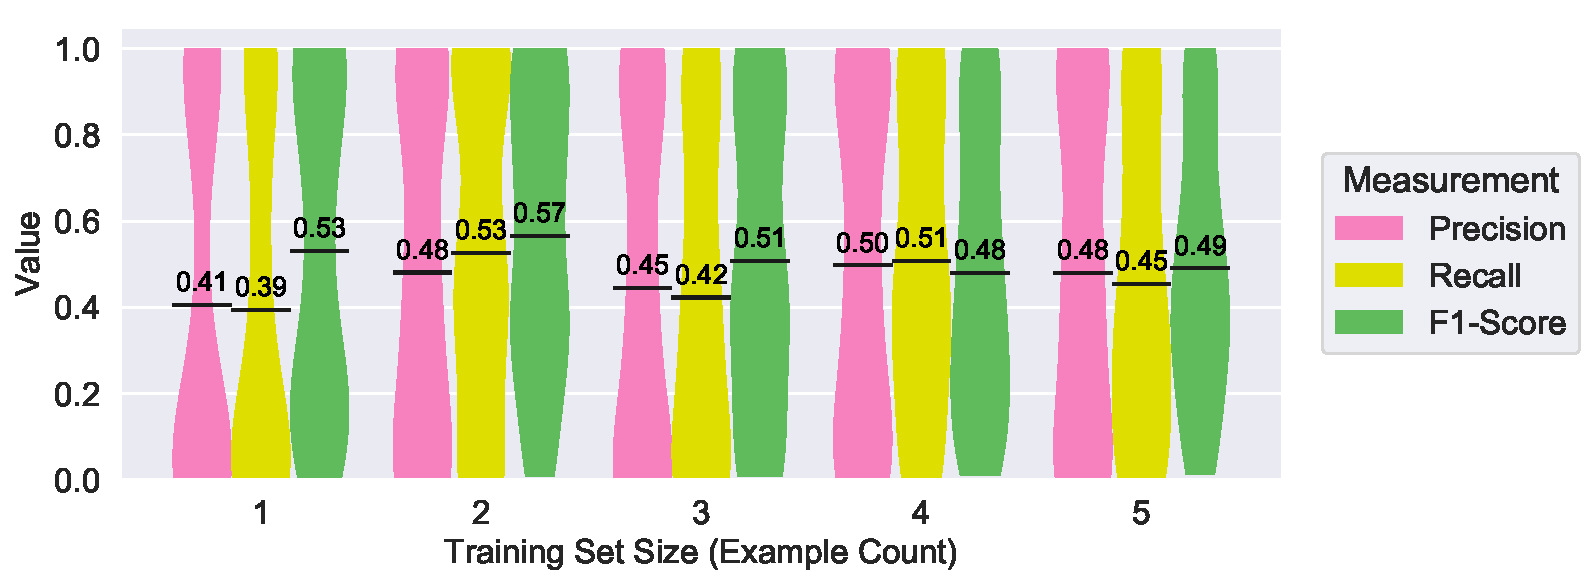
\includegraphics[width=\columnwidth,
		clip]{img/big-study/recall-precision-examplecount-CTS.pdf}
		\caption{Precision, recall and F$_{1}$-score for an
		increasing training set size.}
		\label{fig:recall-precision-examplecount-CTS}

\end{subfigure}\hspace{\fill}
\begin{subfigure}[t]{\columnwidth}
		\centering
				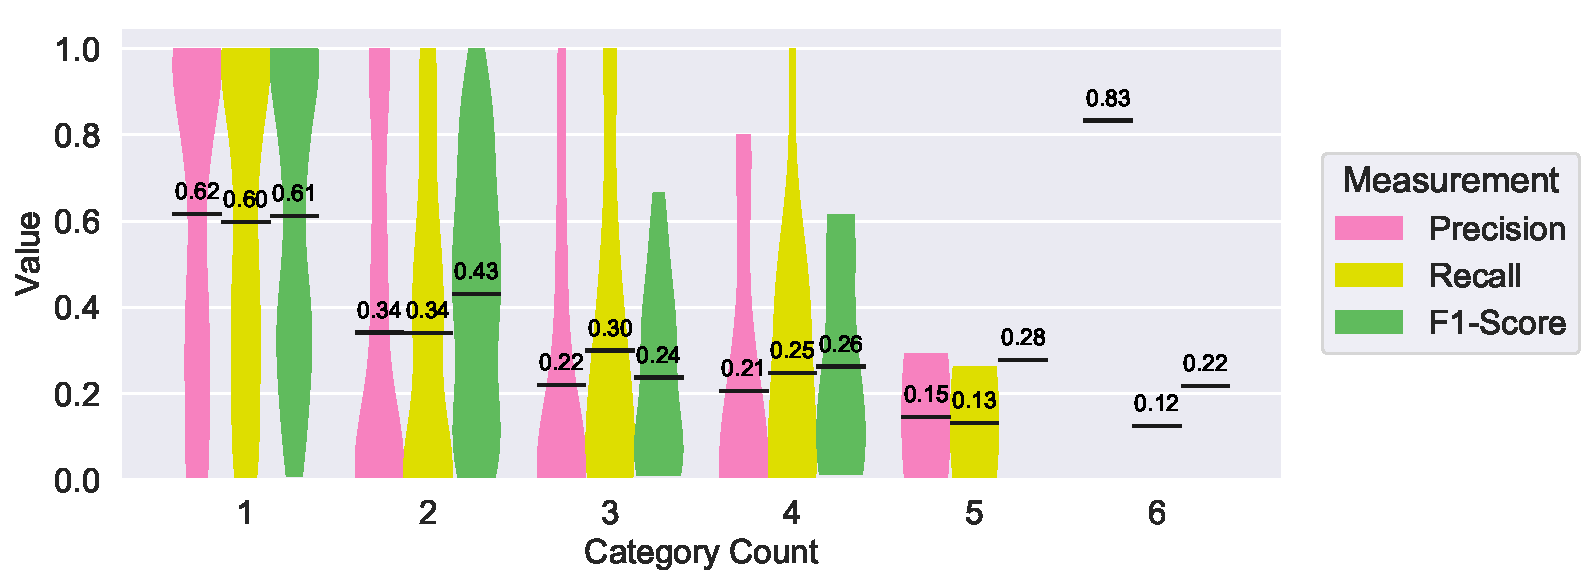
\includegraphics[width=\columnwidth,
				clip]{img/big-study/recall-precision-categorycount-CTS.pdf}
		\caption{Precision, recall and F$_{1}$-score for
		an increasing number of structural categories in the
		training and test sets.}
		\label{fig:recall-precision-categorycount-CTS}
\end{subfigure}
\caption{Results of chunk retrieval with Common Text Similarity (CTS)}
\end{figure*}

\Cref{fig:recall-precision-examplecount-CTS} presents precision,
recall and F$_{1}$-score of chunk retrieval using CTS for an
increasing number of training examples.
When using one to five
training examples, the size of the training set has no noticeable
influence on precision, recall or F$_{1}$-score of the chunk retrieval
with CTS.

\Cref{fig:recall-precision-categorycount-CTS} shows the same
measurements for an increasing number of structural categories in the
training and test examples.
With increasing category count, precision,
recall and F$_{1}$-score decrease.
Especially for more than three
categories present we have no chunk retrieval runs where all desired
lines were extracted.

\subsection{Keyword Search (KWS)}
\label{sec:r:kws}
\begin{figure*}
\centering
    \textbf{Keyword Search (KWS)}\par\medskip
\begin{subfigure}[b]{\columnwidth}
		\centering
		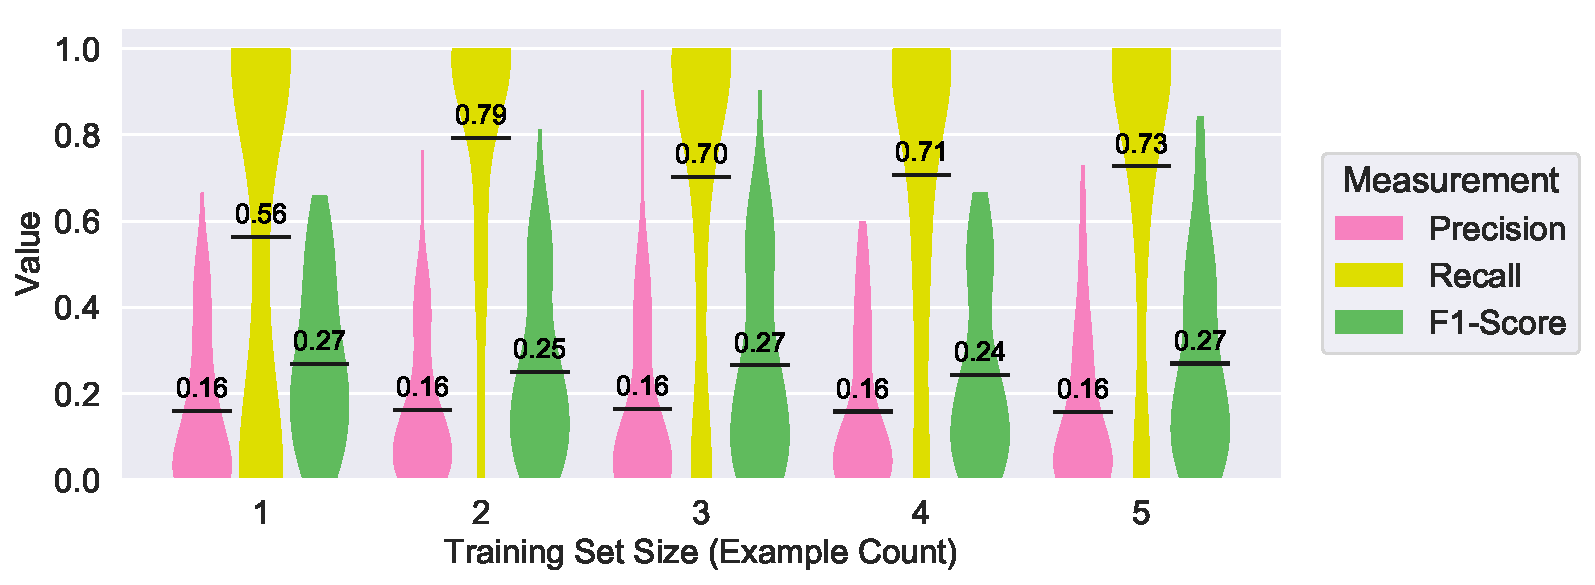
\includegraphics[width=\columnwidth,
		clip]{img/big-study/recall-precision-examplecount-KWS.pdf}
		\caption{Precision, recall and F$_{1}$-score for an
		increasing training set size.}
		\label{fig:recall-precision-examplecount-KWS}
\end{subfigure}\hspace{\fill}
\begin{subfigure}[b]{\columnwidth}
		\centering
		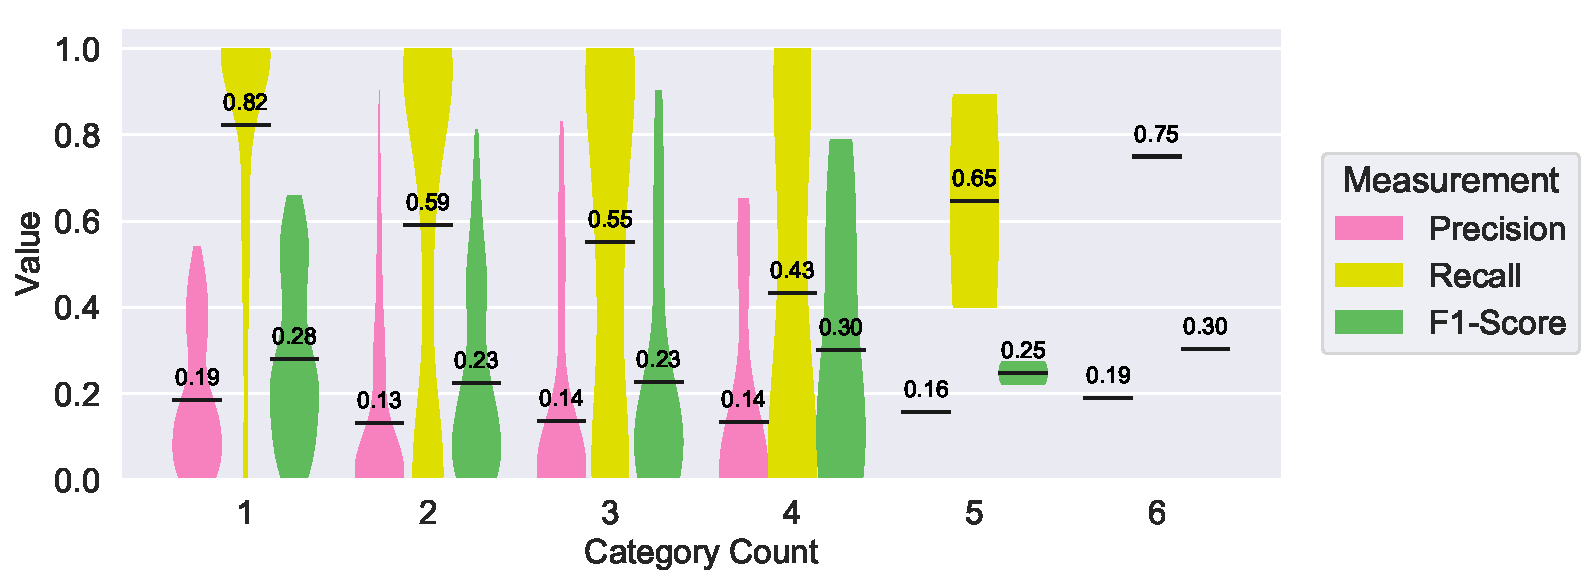
\includegraphics[width=\columnwidth,
		clip]{img/big-study/recall-precision-categorycount-KWS.pdf}
		\caption{Precision, recall and F$_{1}$-score for
		an increasing number of structural categories in the
		training and test sets.}
		\label{fig:recall-precision-categorycount-KWS}
\end{subfigure}
\caption{Results of chunk retrieval with Keyword Search (KWS)}
\end{figure*}


\Cref{fig:recall-precision-examplecount-KWS} presents precision,
recall and F$_{1}$-score of chunk retrieval using KWS for different
numbers of training examples.
The recall increases by about 12\% when
increasing the size of the training set to more than one example,
while the precision stays constant at around 16\%.
The F$_{1}$-score
stays around 26\%.

\Cref{fig:recall-precision-categorycount-KWS} shows the same
measurements for an increasing number of structural categories in the
training and test examples.
For more than one structural category in
the training and test examples the recall decreases by about 20\% and
the precision decreases about 6\%.
For more than two structural
categories no clear trend is visible in precision, recall or
F$_{1}$-score for an increasing amount of categories in the training
and test examples.

% Figure~\ref{fig:contextsizefactor-precision-recall-KWS} shows the
% effect of the retrieval size factor on precision, recall and
% F$_{1}$-score of chunk retrieval runs with KWS\@.
%The precision is
% 19\% when retrieving half of the expected number of lines.
%On
% average 9\% of the lines in the build log are retrieved then.
%When
% 2.5 times the expected number of lines are retrieved, the precision
% decreases to 10\% and a quarter of the lines in the build log are
% retrieved on average.
%The recall ranges from 58\% to 75\% and the
% F$_{1}$-score shows a constant decrease from 29\% to 17\%.

% \begin{figure}[!t]
%		\centering
%		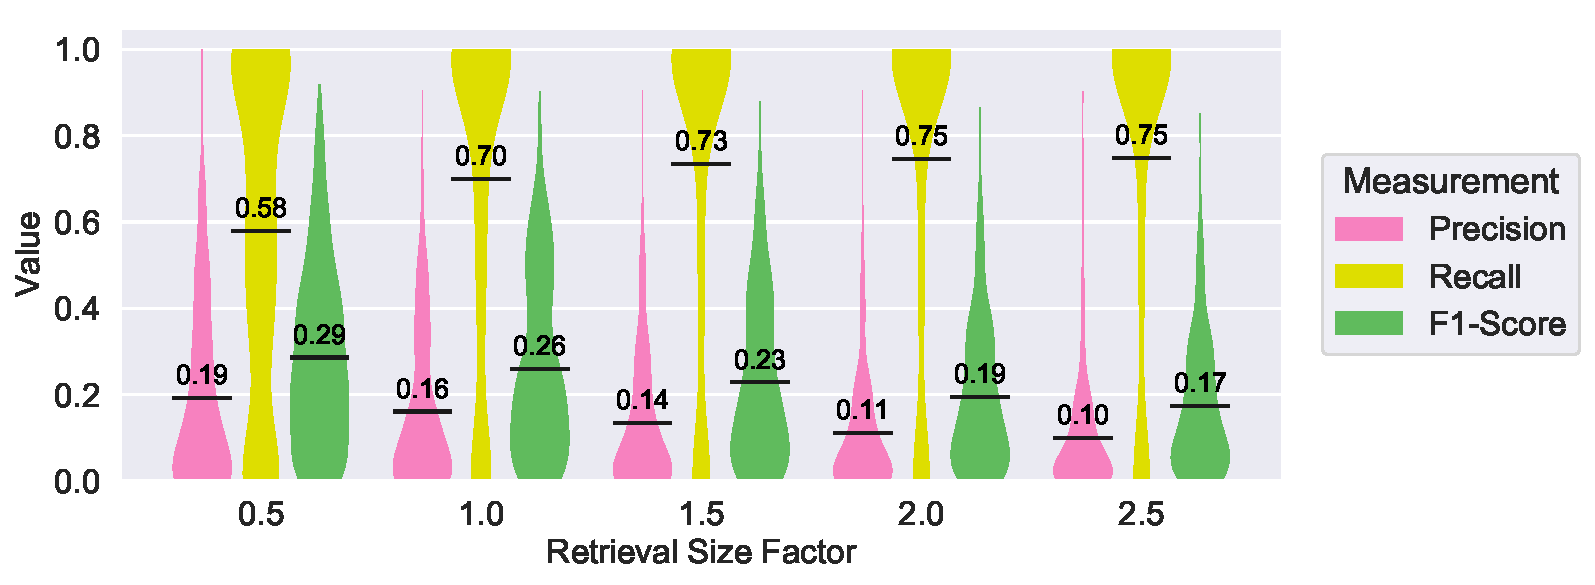
\includegraphics[width=\columnwidth,
%clip]{img/big-study/contextsizefactor-precision-recall-KWS.pdf}
%		\caption{Precision, recall and F$_{1}$-score of chunk
%retrieval with KWS compared to retrieval size factor.}
%		\label{fig:contextsizefactor-precision-recall-KWS}
% \end{figure}

\subsection{Program Synthesis by Example (PBE)}
\label{sec:r:pbe}
\begin{figure*}
\centering
    \textbf{Program Synthesis by Example (PBE)}\par\medskip
\begin{subfigure}[b]{\columnwidth}
		\centering
		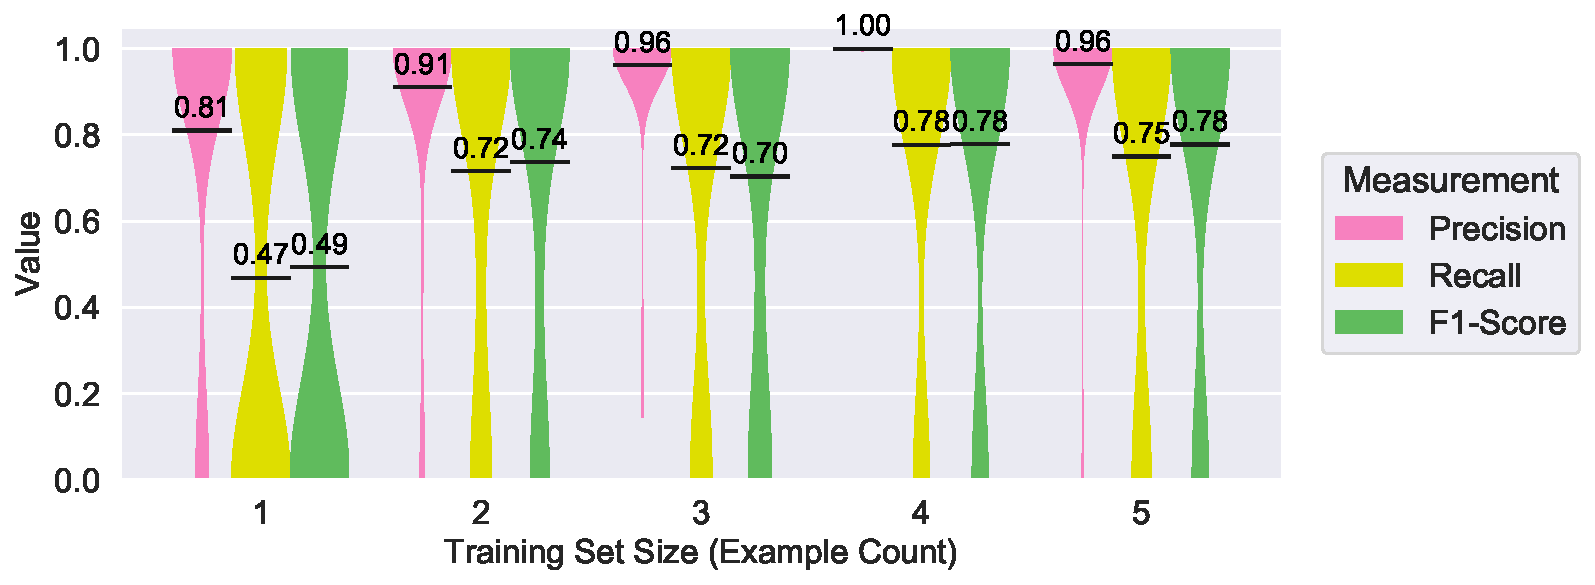
\includegraphics[width=\columnwidth,
		clip]{img/big-study/recall-precision-examplecount-sythesisworked-PBE.pdf}
				\caption{Precision, recall and
				F$_{1}$-score when PBE could synthesize
				a consistent program compared with the
				size of the training set.}
		\label{fig:recall-precision-examplecount-sythesisworked-PBE}
\end{subfigure}\hspace{\fill}
\begin{subfigure}[b]{\columnwidth}
		\centering
		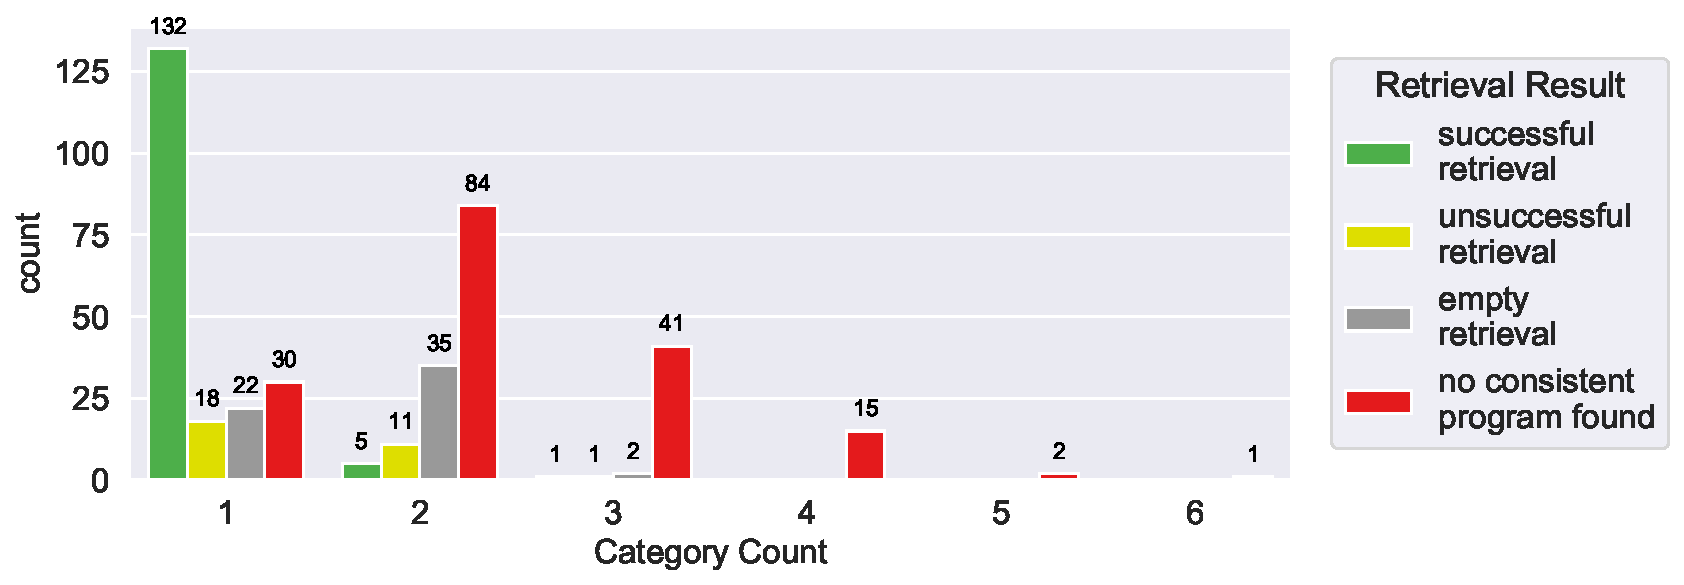
\includegraphics[width=\columnwidth,
		clip]{img/big-study/failure-reason-categorycount-PBE.pdf}
				\caption{Increasing number of structural
				categories in the training and test sets.}
		\label{fig:failure-reason-categorycount-PBE}
\end{subfigure}
\caption{Results of chunk retrieval with  Program Synthesis by Example
(PBE)}
\end{figure*}


\begin{figure}[tbp]
		\centering
		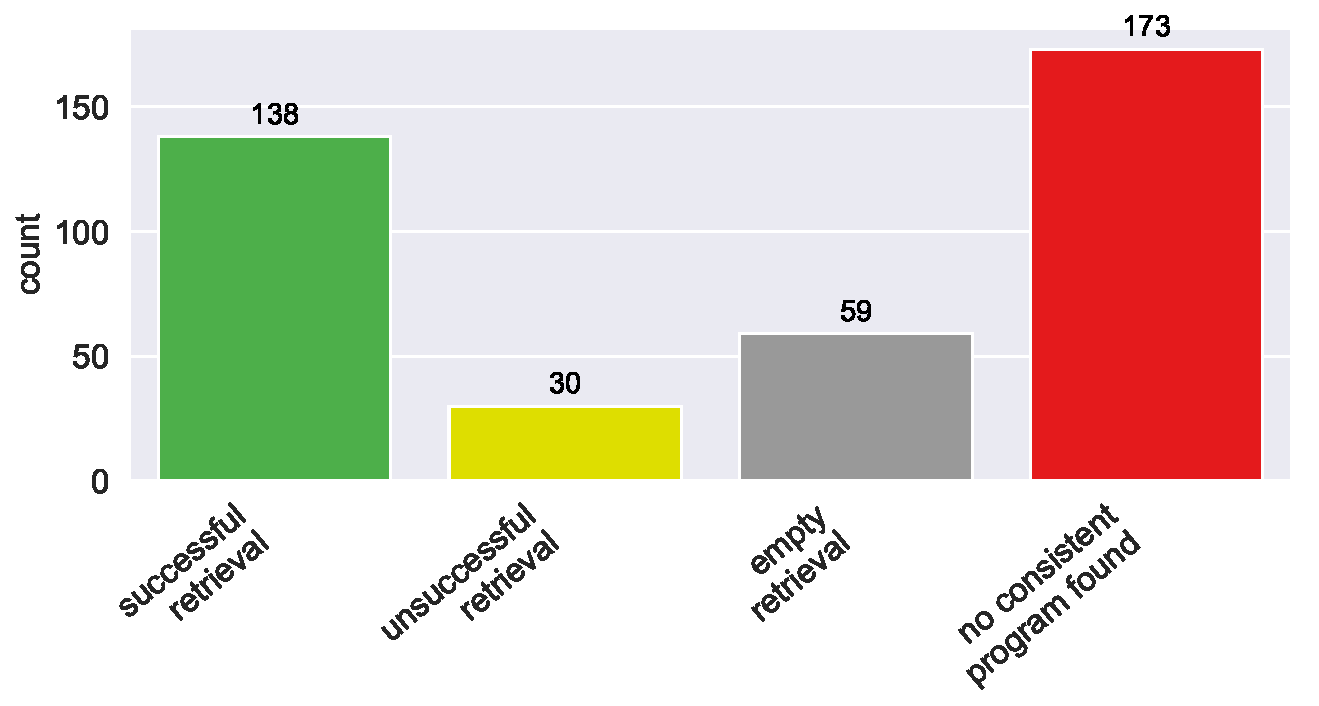
\includegraphics[width=0.75\columnwidth,
		clip]{img/big-study/failure-reason-pbe.pdf}
		\caption{Results of chunk retrieval with PBE.}
		\label{fig:failure-reason-PBE}
\end{figure}

\Cref{fig:failure-reason-PBE} shows the results of the PBE runs in our
evaluation.
Out of the 400 runs, 5 per each one of the 80 example
sets, PBE extracted all the desired lines in 138 cases.
In 89 further
cases, an extraction program was also successfully synthesized, though
in 59 of the 89 cases the synthesized program yielded no output.
In 30
of the 89 cases did the synthesized program only partially extract a
subset of the desired lines.
For these 30 cases, the average recall
was 28\%.
Listing \ref{lst:pbe-unsuccessful} shows an example of such
an \emph{unsuccessful retrieval}, where the synthesized program only
retrieved two of the four targeted lines.
In 173 of the 400 cases
could PROSE not synthesize program consistent with all of the training
examples.

\Cref{fig:failure-reason-categorycount-PBE} shows the results of PBE
runs depend on the number of structural categories in the training and
test examples.
The figure demonstrates that program synthesis mostly
returns exactly the desired output when there are is only one
structural category present in the training examples.
However, when
two or more structural categories are simultaneously present in the
examlpe set, PROSE could in most cases not synthesize a program
consistent with all training examples.
For four or more present
categories PROSE could never synthesize a consistent program.

\Cref{fig:recall-precision-examplecount-sythesisworked-PBE} shows
precision and recall of the 227 runs where PBE could synthesize a
program consistent with all training examples.
When the training set
size increases from one to two, recall and F$_{1}$-score increase by
about 25\%, precision increases by about 10\%.
For two or more
training examples, recall and F$_{1}$-score stay around 75\% and
precision around 96\%.

\subsection{Random Line Retrieval}
\label{sec:r:rlr}

In our evaluation, we compare against a baseline of randomly
picking lines from the build log.
Its results follow intuitive
expectations:
The precision ranges between 8\% and 5\%, the recall between 6\% and
8\%.
The size of the training set has no visible impact on either.
An greater number of structural categories within the training and
test sets decreased the precision of RLR from 7\% to 0\%, the recall
increases from 6\%, for one structural category present, to 11\%, for
three sturctural categories present and also drops to 0\% for more
structural categories.
Graphs of the results of the chunk retrieval with RLR from our study
are included in our replication
package~\cite{brandt2020chunk-replication}.


\subsection{Comparison of All Techniques}
In this section, we aggregate the results from
\Cref{sec:r:kws,sec:r:pbe,sec:r:cts,sec:r:rlr} and put them next to it
each other.

\Cref{fig:success-partial-all} compares the success of chunk
retrievals differentiated by techniques in our study.
CTS and KWS
extract some of the desired lines in 79\% and 88.5\% of the chunk
retrieval runs.
With 38.25\%, KWS also has the highest number of fully
successful extractions, followed by PBE with 34.5\%.
PBE has the
lowest number of partial retrievals with only 18 out of 400 chunk
retrieval runs.

% The averaged precision, recall and F$_{1}$-score f all techniques is
% compared in Figure~\ref{fig:recall-precision-all}.
The recall of PBE
% has a high skew towards one and zero, meaning in most cases either
% the retrieval is successful or no relevant lines are extracted at
% all.
PBE has the highest average precision with 95\%.
Chunk
% retrieval with CTS has the highest average F$_{1}$-score with 51\%
% and the second highest recall with 46\%.
KWS has the smallest
% precision of the three chunk retrieval techniques.
With 16\% it is
% still higher than the precision of the RLR baseline with 7\%.
KWS
% has the highest recall of all techniques with 70\%.

\Cref{fig:recall-precision-singlecategory-all,fig:recall-precision-multicategory-all}
show the influence of a single structural category present in the
training examples compared to multiple categories present.
For more
than one category being present, the recall of PBE decreases greatly.
For CTS and KWS the values also decrease, while RLR is not affected by
the number of structural categories present.

\begin{figure}[!t]
		\centering
		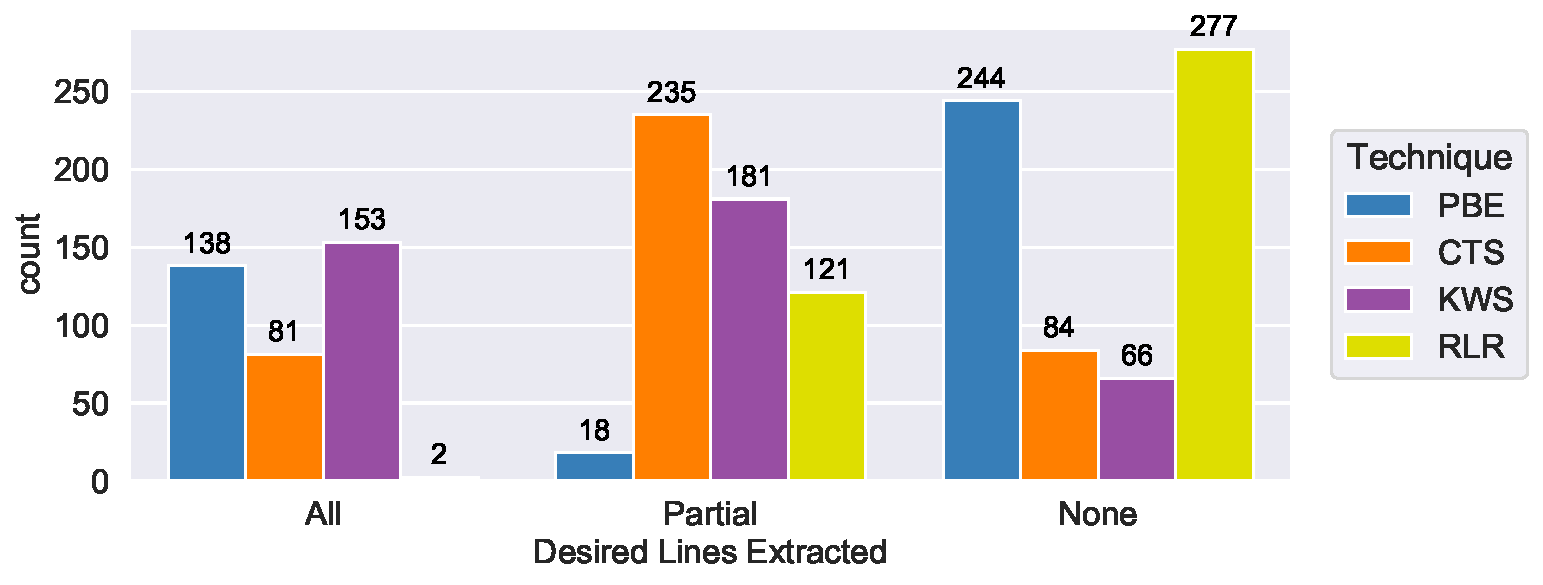
\includegraphics[width=\columnwidth,
		clip]{img/big-study/success-partial-all.pdf}
		\caption{Success of chunk retrievals for all techniques.}
		\label{fig:success-partial-all}
\end{figure}

\begin{figure*}
\centering
    \textbf{PBE, CTS, KWS, and RLR}\par\medskip
\begin{subfigure}[b]{\columnwidth}
		\centering
				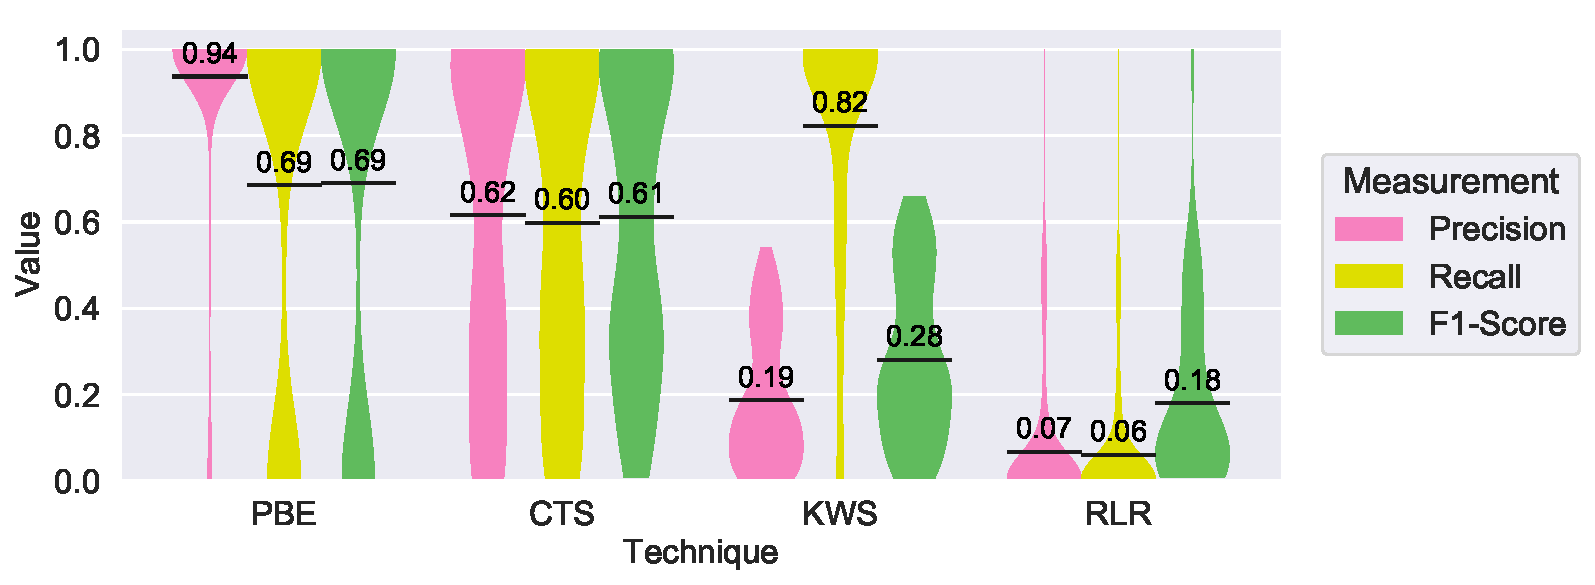
\includegraphics[width=\columnwidth,
				clip]{img/big-study/recall-precision-singlecategory-all.pdf}
		\caption{Precision, recall and F$_{1}$-score of all
		techniques when training examples are in \emph{one}
		structural category.}
		\label{fig:recall-precision-singlecategory-all}
\end{subfigure}\hspace{\fill}
\begin{subfigure}[b]{\columnwidth}
		\centering
				\centering
		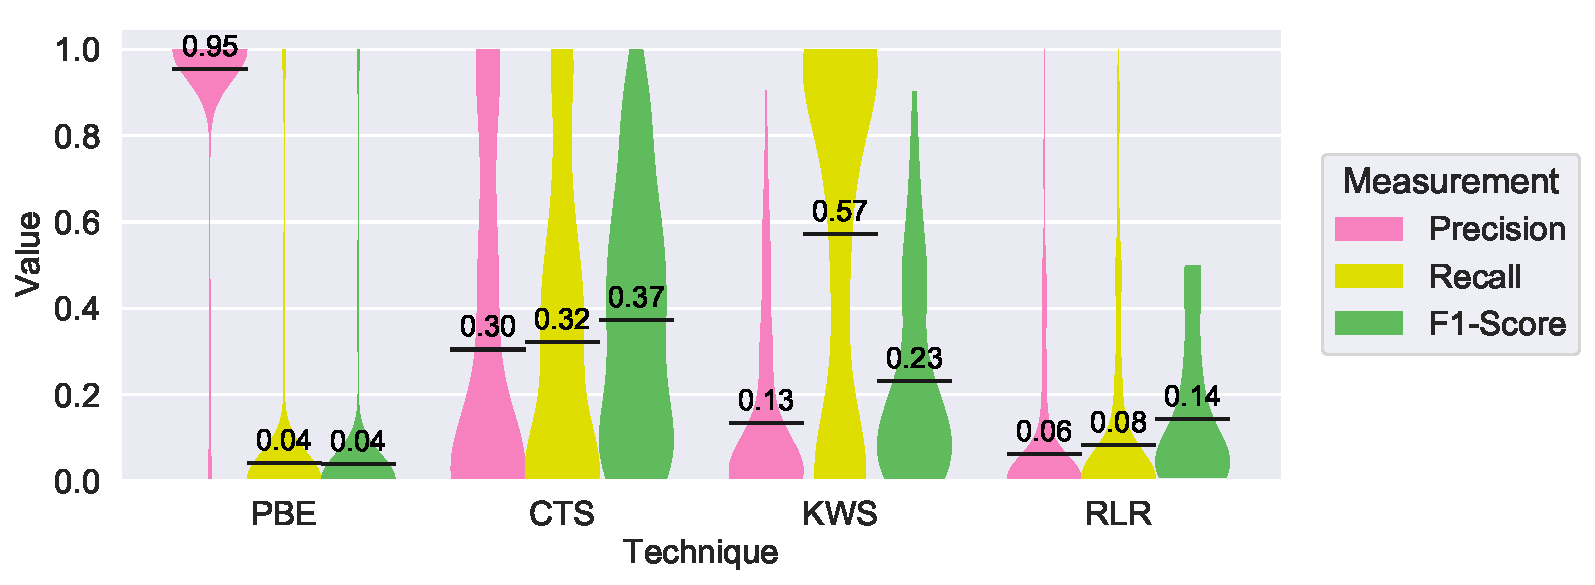
\includegraphics[width=\columnwidth,
		clip]{img/big-study/recall-precision-multicategory-all.pdf}
		\caption{Precision, recall and F$_{1}$-score of all
		techniques when training examples are in \emph{more than
		one} structural categories.}
		\label{fig:recall-precision-multicategory-all}
\end{subfigure}
\caption{Comparison of all chunk retrieval techniques, split by structural
category count.}
\end{figure*}

\section{Discussion}
\label{sec:discussion}

% TODO update RQs
% TODO incorporate these RQs into the text where they are being answered

This section presents the answers to our research questions:
\begin{simplebox}{Research Questions}
\begin{itemize}
  \item[\textbf{RQ1:}] Which build log analysis techniques exist?
  \item[\textbf{RQ2:}] Which criteria influence the suitability of a
  chunk retrieval technique for build logs?

  {\small \item[\textbf{~~ RQ2.1:}] How many examples do PBE, CTS,
  and KWS need to perform best?
  \item[\textbf{~~ RQ2.2:}] How structurally similar do the examples
  for PBE, CTS and KWS need to be for the techniques to be applicable?
  \item[\textbf{~~ RQ2.3:}] How accurate are the retrievals of PBE, CTS,
  and KWS?}
\end{itemize}
\end{simplebox}

The first section discusses for PBE, CTS and KWS separately in which
cases they perform best.
It details for which types of input build
logs, available training examples and consumption of the retrieved
output each technique is suited.
In the following section we discuss
which of these criteria should influence the decision to use a certain
technique most.
Based on our empirical comparison, we present a
decision tree between the three techniques we investigated.

\subsection{Interpretation of Study Results}
This section discusses the study results for each of the analyzed
chunk retrieval techniques separately.
It gives recommendations which
kind of information chunk targets are best for each technique and for
what kind of usage the respective output is suitable.

\begin{table}[tbp]
\resizebox{\columnwidth}{!}{%
\centering
\begin{tabular}{llll}
  \toprule
  & PBE & CTS & KWS \\
  \midrule
  Structural Categories & 1 & less is better & \makecell[l]{best 1 \\
  multiple okay} \\
  Training Set Size & 2 & no influence & 2 \\
  Precision & \makecell[l]{high \\ (if synthesis succeeds)} & medium &
  low \\
  Recall & \makecell[l]{high \\ (if synthesis succeeds)} & medium &
  high \\
  \makecell[l]{Confidence in \\ Output Correctness} & high & low &
  \makecell[l]{low (precision) \\ high (recall)} \\
  Output Consumption by & program & human & human \\
  \bottomrule
\end{tabular}%
}
\caption{Recommendations for each of the investigated chunk retrieval
techniques.}
\label{tab:single-technique-recommendations}
\end{table}

\subsubsection{Program Synthesis by Example (PBE)}

\noindent
\textbf{Configuration and Input}
Our study results show that chunk retrieval with PBE gives best
results when the training examples are structurally identical.
This is
because PROSE has difficulty synthesizing OR-based programs (see
\Cref{sec:prose:impl}).
PBE is thus suited to retrieve information
chunks that always have the same surrounding or defining internal
structure.
To extract for example the reason a build failed, the log
passage describing the failure would always have to be started and
ended the same way.

When the training examples are of the same structure, even one or two
two examples are enough input for PROSE to synthesize a regular
expression program with good recall.
In our study, additional training
examples did not improve the chunk retrieval.
In fact, unless they
were in some sense redudant, adding training examples above that even
hindered the applicability of PBE.

\noindent
\textbf{Retrieval Output Usage}
If the program synthesis succeeds and applying the regular expression
program yields an output, PBE has high precision and recall.
The tool
clearly identifies a failing program synthesis or when no output from
the program applied to a build log is obtained.
Therefore, if there is
an output, the user can have high confidence that it is the desired
output.
This preciseness makes output from PBE chunk retrieval
well-suited for machine consumption.

\subsubsection{Common Text Similarity (CTS)}
\noindent
\textbf{Configuration and Input}
Similar to PBE, chunk retrieval using CTS yields better results the
fewer structural categories are present in the training and test
examples.

The number of training examples had no noticeable influence on
precision or recall in our study.
Information retrieval techniques
like text similarity commonly learn on a higher number of examples
than used for our study.
Future work is needed to investigate how many
examples yield improvements in the chunk retrieval over a single
training example.

\noindent
\textbf{Retrieval Output Usage}
CTS has good precision and recall on average, though with a high
variation.
This means that the quality of an output by CTS is hard to
determine, which makes it unsuited for automatic  processing and requires
a human to further inspect and interpret the output.
This could include semi-automated procedures such as sending
developers an email with the extracted build failure reason.

\subsubsection{Keyword Search (KWS)}
\noindent
\textbf{Configuration and Input}
KWS has a higher recall than the two other techniques for multiple
structural categories present in the training and test examples.
This
makes KWS a good technique if there is little prior knowledge on how
the targeted log chunk is represented in the build log.
For the
example of extracting the reason the build failed, KWS is best suited
if a build can fail in various steps logged by different tools and no
pre-categorization of where the build failed is available.

Going from one to two two training examples, KWS's recall improves
siginficantly.
However, further enlarging the training example count
does not lead to further improvments.

Retrieving the average number of lines present in the outputs of the
training examples around every found keyword yields reasonable recall.
Selecting 1.5 times as many lines around every found keyword does
improve the recall within our study but also increases the proportion
of lines retrieved overall and therefore decreases precision.

\noindent
\textbf{Retrieval Output Usage}
While KWS has the highest recall of all three techniques, its
precision is the lowest.
The output of a chunk retrieval with KWS is
well-suited to be read by humans, but ill-suited for consumption by
automated tools.

\begin{figure}[tb]
		\centering
		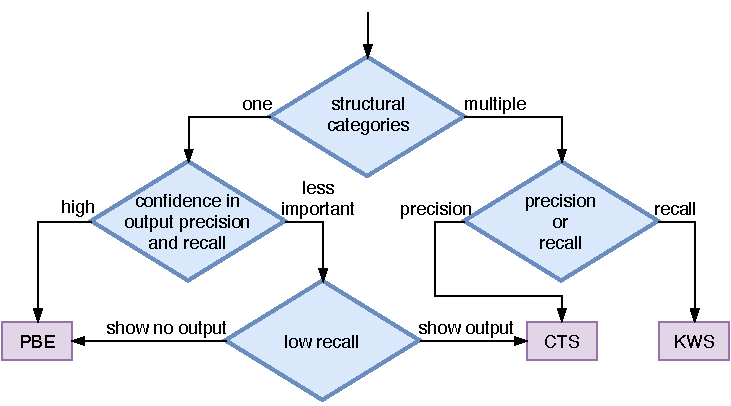
\includegraphics[width=\columnwidth,
		clip]{img/crt-recommendation.pdf}
		\caption{Our preliminary recommendation scheme for chunk
		retrieval techniques.}
		\label{fig:crt-recommendation}
\end{figure}

\subsection{Recommendation of Suitable Techniques}
After discussing the three chunk retrieval techniques separately we
now want to unify our results into one recommendation scheme.
In
Figure~\ref{fig:crt-recommendation}, we present a decision tree, which
developers and researchers who want to retrieve information chunks
from build logs can follow.
The decision tree is built up of questions
which either lead to more questions or to a leaf node containing a
recommended technique.


\noindent
\textbf{Caveat!} This is a preliminary hypothesis based on the results
from our comparison study.
The recommendations could therefore be
influenced by idiosyncrazies of our specific implementation of the
chunk retrieval techniques as well as the logs in the \emph{LogChunks}
data set.

This decision tree in \Cref{fig:crt-recommendation} gives a nunanced
answer to RQ2, about which criteria influence the suitability of a
chunk retrieval technique.
The earlier in the decision tree a
criterion is noted, the more important it is when distinguishing the
techniques.

The first and most important aspect are the structural categories.
Are
the information chunks one would like to retrieve always presented in
the same structural way within the build logs? Then the information
chunks in all training examples and the analyzed build log are in the
same structural category.

If the information chunks are from multiple structural categories,
i.e.
they are not represented in the same structural way within the
build logs, and recall is more important than precision we recommend
to use KWS\@.
If the representations are from multiple structural
categories and precision is more important than recall to the user we
recommend CTS\@.
We also recommend CTS when the representations are
from one structural category, when the user does not require a high
confidence in the precision or recall of the outcome and when the user
would rather have output with low recall instead of no output at all.
When the representations are from one structural category and the user
wishes a high confidence in the correctness of the output or prefers
no output over output with low recall, we recommend PBE\@.

As a final recommendation, one could create a ``super analyzer'' by
combining the different build log analysis techniques studied in this
paper.
Such a super analyzer would likely always first employ PBE
(because of its high accuracy), followed by a combination of CTS and
KWS.
Other than initial setup and training time, there should be no
downside to this approach if it is implemented in a transparent way to
the underlying technique: the output of the super analyzer could
include from which sub-tool it originated and thus facilitate
automatic on-ward processing or interpretation of the result.


\noindent
\textbf{Example of Using the Recommendation Scheme}
To illustrate how one would use our decision tree to find a suitable
chunk retrieval technique we describe two concrete examples: a
researcher investigating why CI builds fail and a software team
wanting to monitor their build performance.

In our first example, a researcher studies whether test failures in CI
are caused by a small or by a large group of test cases.
They gather
CI build logs from various projects, which are their only available
data source.
The task of the researcher is to extract the names of the
failing test cases from each build log.
When they use our
recommendation scheme to select a chunk retrieval technique, they
first have to estimate how uniform the representation of the failing
test cases is in the investigated build logs.
As the researcher is
covering a wide range of build tools and development languages, the
log chunks they target are in various, non-predictable structural
representations.
The next question is whether they value precision
over recall.
As they have to manually inspect the results of both CTS
and KWS, they choose recall over precision to avoid having to inspect
the whole log in case the relevant information chunk was not
retrieved.
Therefore, our decision tree recommends them to use KWS\@.

In case the researcher wants to avoid manually inspecting the
retrieval results, they have to first separate the CI build logs
according to the test tool responsible for logging the test results.
Then the targeted log chunks are from one structural category and they
can use PBE, trained with examples from each test tool separately.

In our second example, a software development team wants to monitor
the performance of the phases within their CI build.
They are using
Travis CI, which measures the duration of build phases and documents
them within the build log.
As all log statements that report timing
measurements are formatted the same way, the targeted log chunks are
from one structural category.
Therefore the development team can use
PBE to retrieve the duration of a build phase as well as its name.

\section{Threats to Validity}
There are several threats to the validity of the conclusions of our
work.

\noindent
\textbf{Implementation}
\label{sec:prose:impl}
% TODO we need to say something about why we think that these
% limtiations do not actually harm our results
Our results depend on the implementation of the investigated chunk
retrieval techniques and the libraries we used.
Our implementation of
PBE is based on the program synthesis provided by PROSE\@.
The
idiosyncrazies of this framework influence our PBE results.
Other
frameworks similar to PROSE might have somewhat different strengths
and weaknesses.
For example, the need for examples from a single
structural category stems from the fact that PROSE cannot learn
regular expression programs with arbitrary boolean conjunctions and
disjunctions~\cite{mayer2015user}.
PROSE introduced this constraint to
keep the synthesis performance reasonable.
At the same time, this is
clearly a current theoretical challenge of all PBE implementations,
and we therefore attribute it to the technique itself, rather than the
specific implementation.

% TODO cite http://text2vec.org/
Our implementation of CTS is dependent on the library {\tt text2vec}
and the way it splits strings into word tokens.
On the other hand,
{\tt text2vec} is the de-facto standard library to do word embeddings
in R.
We intentionally chose a simple, minimally configured and tuned
approach to compare against.
Tuning the text similarity
meta-parameters more to the specific use case of chunk retrieval from
build logs would yield better chunk retrieval results.

\noindent
\textbf{Data Set}
The outcomes of our comparison study are highly dependent on the build
logs from the \emph{LogChunks} data set.
It only consists of build
logs from open source projects and therefore it is not clear whether
our results are generalizable to industry projects.
We only collected
build logs from Travis CI, however we chose to evaluate on an
information chunk whose format is not dependent on Travis CI\@.
This
is because the reason the build failed is described within the build
logs by the tools themselves and not the Travis CI environment.

\noindent
\textbf{Training Set Size}
Especially the results for CTS might be influenced by the fact that we
only trained on one to five examples.
We chose this small training set
size as the training examples have to be provided per repository and
we expect a developer to not want to provide more examples than the
small numbers we evaluated on.

\noindent
\textbf{Few Samples with Many Structural Categories}
Our comparison study shows fewer measurements with many structural
categories than with one category.
This stems from the fact that we investigated the chunk retrieval
techniques on a realistic data set, which showed to often have few
structural categories within one project.

\section{Future Work}
\todo{survey build logs tools in industry}

There are various future research opportunities based on our work:
\begin{itemize}
  \item \textbf{Further Analysis of \emph{LogChunks}} We created the
  \emph{LogChunks} data set \cite{brandt2020logchunks} specifically for
  the comparative
  study in this paper, though it can be the basis for various further
  analyses of build log data.
The keywords, for example, can be
  investigated to answer which keywords are used to search for the
  reason the build failed within build logs.
  \item \textbf{Cross-Repository Build Log Analysis} We trained and
  tested each chunk retrieval technique on examples from the same
  repository.
We propose to analyze how techniques could be trained
  across repositories, building the cornerstones for build
  environment-agnostic analysis tools.
  \item \textbf{Comparison with more Chunk Retrieval Techniques} This
  paper investigates the three chunk retrieval techniques PBE, CTS and
  KWS\@.
Our study design can be reused to evaluate other build log
  analysis techniques, such as the diff and information retrieval
  approach by Amar et al.~\cite{amar2019mining}.
  \item \textbf{Refinement of Retrieval Quality for each Technique} We
  investigated basic configurations of existing techniques applied to
  chunk retrieval from build logs.
In a next step, each of these
  techniques could be refined to better approach the domain of build
  logs.
The \emph{LogChunks} data set and our study results act as a
  baseline to benchmark such technique improvements.
We propose the
  following improvements:
    \begin{itemize}
      \item \textbf{Custom Ranking and Tokens for PBE} The program
      synthesis through PROSE ranks possible programs according to
      what the user most likely intended.
One could adapt the ranking
      rules provided by the FlashExtract DSL to fit common build log
      chunk retrieval tasks.
FlashExtract includes special tokens when
      enumerating possible regular expressions.
One could extend these
      with tokens found in build logs, such as ``-'',``='',``ERROR''
      or ``[OK''.
      \item \textbf{Meta-Parameter Optimization for CTS} Information
      retrieval techniques have various meta-parameters which can be
      optimized for the specific use
      case~\cite{panichella2016parameterizing}.
We propose to further
      investigate improvements in preprocessing of the log text, in
      tokenization of the log lines into terms and in stop words
      lists.
    \end{itemize}
  \item \textbf{Usability Analysis of Chunk Retrieval Output} Our
  analysis of the output produced by the chunk retrieval focuses on
  precision and recall.
We propose to investigate how useful these
  outputs are to developers through controlled experiments.
\end{itemize}


\section{Conclusion}
\label{sec:conclusion-fw}
The goal of this paper was to support researchers and developers in
their decision on how to analyze build logs. We implemented and
compared three different chunk retrieval techniques on our data set
\emph{LogChunks}, composed of 797 manually labeled build logs from a
broad range of 80 repositories. Our results show that the structural
representation of the targeted information in the build logs is the
main factor to consider when choosing a suitable technique. Secondary
factors are the desired confidence into recall and precision of the
produced output and whether precision or recall is more important for
the task at hand.

As a final recommendation, one could create a ``super analyzer'' by
combining the different build log analysis techniques studied in this
paper. 
